\documentclass{beamer}

\usepackage{beamerthemesplit}
\usepackage[german]{babel}
\usepackage[T1]{fontenc}
\usepackage[latin1]{inputenc}
 

\title{autoBAHN - Ultraschallsensoren}
\author{Angel Mirkovski, Martin Schneider}
\institute{Universit�t Salzburg \\Softwarepraktikum 2009/10}
\date{\today}

\begin{document}
\setbeamertemplate{footline}{
    \begin{beamercolorbox}[wd=0.5\textwidth,ht=3ex,dp=1.5ex,leftskip=.5em,rightskip=.5em]{author in head/foot}
        \usebeamerfont{author in head/foot}
        \hfill\insertshortauthor
    \end{beamercolorbox}
    \vspace*{-4.5ex}\hspace*{0.5\textwidth
    }\begin{beamercolorbox}[wd=0.5\textwidth,ht=3ex,dp=1.5ex,left,leftskip=.5em]{title in head/foot}
        \usebeamerfont{title in head/foot}
        \insertshorttitle
        \hfill\insertframenumber/\inserttotalframenumber
    \end{beamercolorbox}
}
\frame{\titlepage}
\frame{}
\section{Ultraschallsensor}
\frame
{
  \frametitle{Ultraschallsensor}
 
  \begin{center}
  	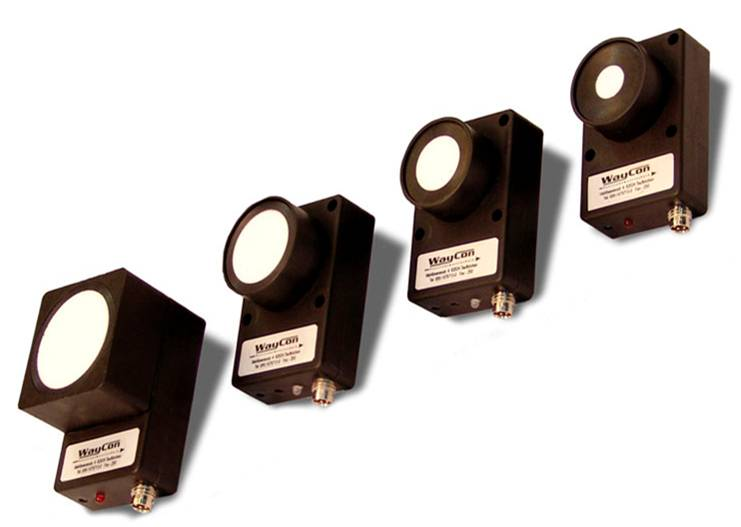
\includegraphics[scale=0.4]{sensor.jpg}
  \end{center}
  \begin{itemize}
  \item<1-> Waycon UN-5000 (\url{www.waycon.de})
  \item<2-> Messbereich: ca. $400-5000 mm$
  \item<3-> Ausgabe: $0\dotsc10V (1 \sim 50 mm)$
  \end{itemize}
}
\frame
{
  \frametitle{Ultraschallsensor}
  \begin{itemize}
  \item<1-> Schutzklasse IP67
  	\begin{itemize}
  		\item<2-> gegen Ber�hrung
  		\item<3-> gegen Eindringen von Staub
  		\item<4-> gegen Wassereindringen bei zeitweisem Untertauchen
  	\end{itemize}
  \item<5-> Funktionweise: Laufzeitmessung von Schallwellen
  \end{itemize} 
}
\section{A/D - Wandler}
\frame
{
  \frametitle{A/D-Wandler}
  \begin{center}
  	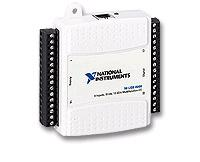
\includegraphics[scale=0.6]{umwandler.jpg}
  \end{center}
  \begin{itemize}
  \item<1-> National Instruments NI 6008 USB (\url{www.ni.com})
  \item<2-> macht die Messdaten des Sensors �ber USB lesbar
  \item<3-> Analoge und digitale Ein- und Ausg�nge
  \end{itemize}
}
\frame
{
  \frametitle{A/D-Wandler (Fortsetzung)}
  \begin{itemize}
  \item<1-> 8 analoge und 4 digitale Eing�nge
  \item<2-> input range $\pm10 V$ f�r analoge und $\pm20, \pm10, \pm5, \pm4, \pm2.5, \pm2, \pm1.25, \pm1 V$ f�r die digitalen
  \item<3-> Maximum working voltage ist $\pm10 V$
  \item<4-> Overvoltage protection ist $\pm35 V$
  \item<5-> 2 analoge Ausg�nge
  \item<6-> Output range $0$ $to$ $5 V$
  \end{itemize}
}
\frame
{
  \frametitle{A/D-Wandler (Fortsetzung)}
  \begin{itemize}
  \item<1-> Treiber f�r Windows, Linux und Mac OS X
  \item<2-> Empfohlende Software - LabVIEW, LabWindows/CVI, Measurement Studio
  \item<3-> Andere Software - C\#, Visual Basic .NET und ANSI C
  \item<4-> Verwendete Treiberversion: NIDAQmx Base 3.3 f�r Windows
  \end{itemize}
}
\section{Sensor.dll}
\frame
{
  \frametitle{Sensor.dll}
  \begin{itemize}
  \item<1-> Simples C-Program, das Methoden zum Lesen eines analogen Eingangs vom NI USB A/D-Wandler bietet.
  \item<2-> Schnittstelle zwischen Treiber und unserer Java-Software
  \end{itemize}
}
\section{JNI und JAW}
\frame
{
  \frametitle{JNI und JAW}
  \begin{itemize}
  \item<1-> JNI - Java Native Interface
  \item<2-> JAW - Jave API Wrapper (\url{www.aplu.ch/jaw})
  \item<2->
  \item<3-> Erm�glichen das Ausf�ren von nativem C-Code in Java-programmen
  \item<4-> Verwendung: Aufruf der sensor.dll und Zugriff auf den Sensor aus dem Java-Programm
  \end{itemize}
}
\section{Unser Programm}
\frame
{
  \frametitle{Unser Programm}
  \begin{itemize}
  \item<1-> Verwaltung und Visualisierung von Ultraschallsensoren
  \item<2-> Objektorientierter Ansatz (Sensor, UltraSonicSensor, DetectedObject, ...)
  \item<3-> Observer-Pattern (Sensor-GUI wird nur neu gezeichnet, wenn sich Daten �ndern)
  \item<4-> Das GUI ist wie alles anderen Komponenten f�r den Betrieb mit mehreren (auch unterschiedlichen) Sensoren vorgesehen
  \end{itemize}
}
\end{document}
